\documentclass[../main.tex]{subfiles}
\graphicspath{{\subfix{../images/}}}


\begin{document}
% AIS
%%%%%%%%%%%%%%%%%%%%%%%%%%%%%%%%%%%%%%%%%%%%%%%%%%%%%%%%%%%%%%%%%%%%%%%%%%%%%%%
Vessels navigating the Baltic Sea

Importance of maritime traffic globally and timely operation


\subsection{Automatic identification system}

What is AIS, what is is features, problems. Example of raw AIS data.

Type A and B message types

\subsubsection{Estimated Time of Arrival}

Importance of ETA and what current systems there is.

\subsection{HELCOM dataset}

Introduction to HELCOM

Describe the features and quirks with the HELCOM dataset as it is a processed dataset that contains AIS data already processed from the raw format. Merging of A and B AIS message types

HELCOM dataset has no ETA entries meaning to use this dataset for ETA prediction the ATA is calculated for all points on the route until the vessel has arrived, the true arrival time. Can't compare vessels ETA with the estimation but knows the estimated time left 

Showing examples of the data as plots of the Baltic, also shows the area covered

\begin{figure}[h]
\centering
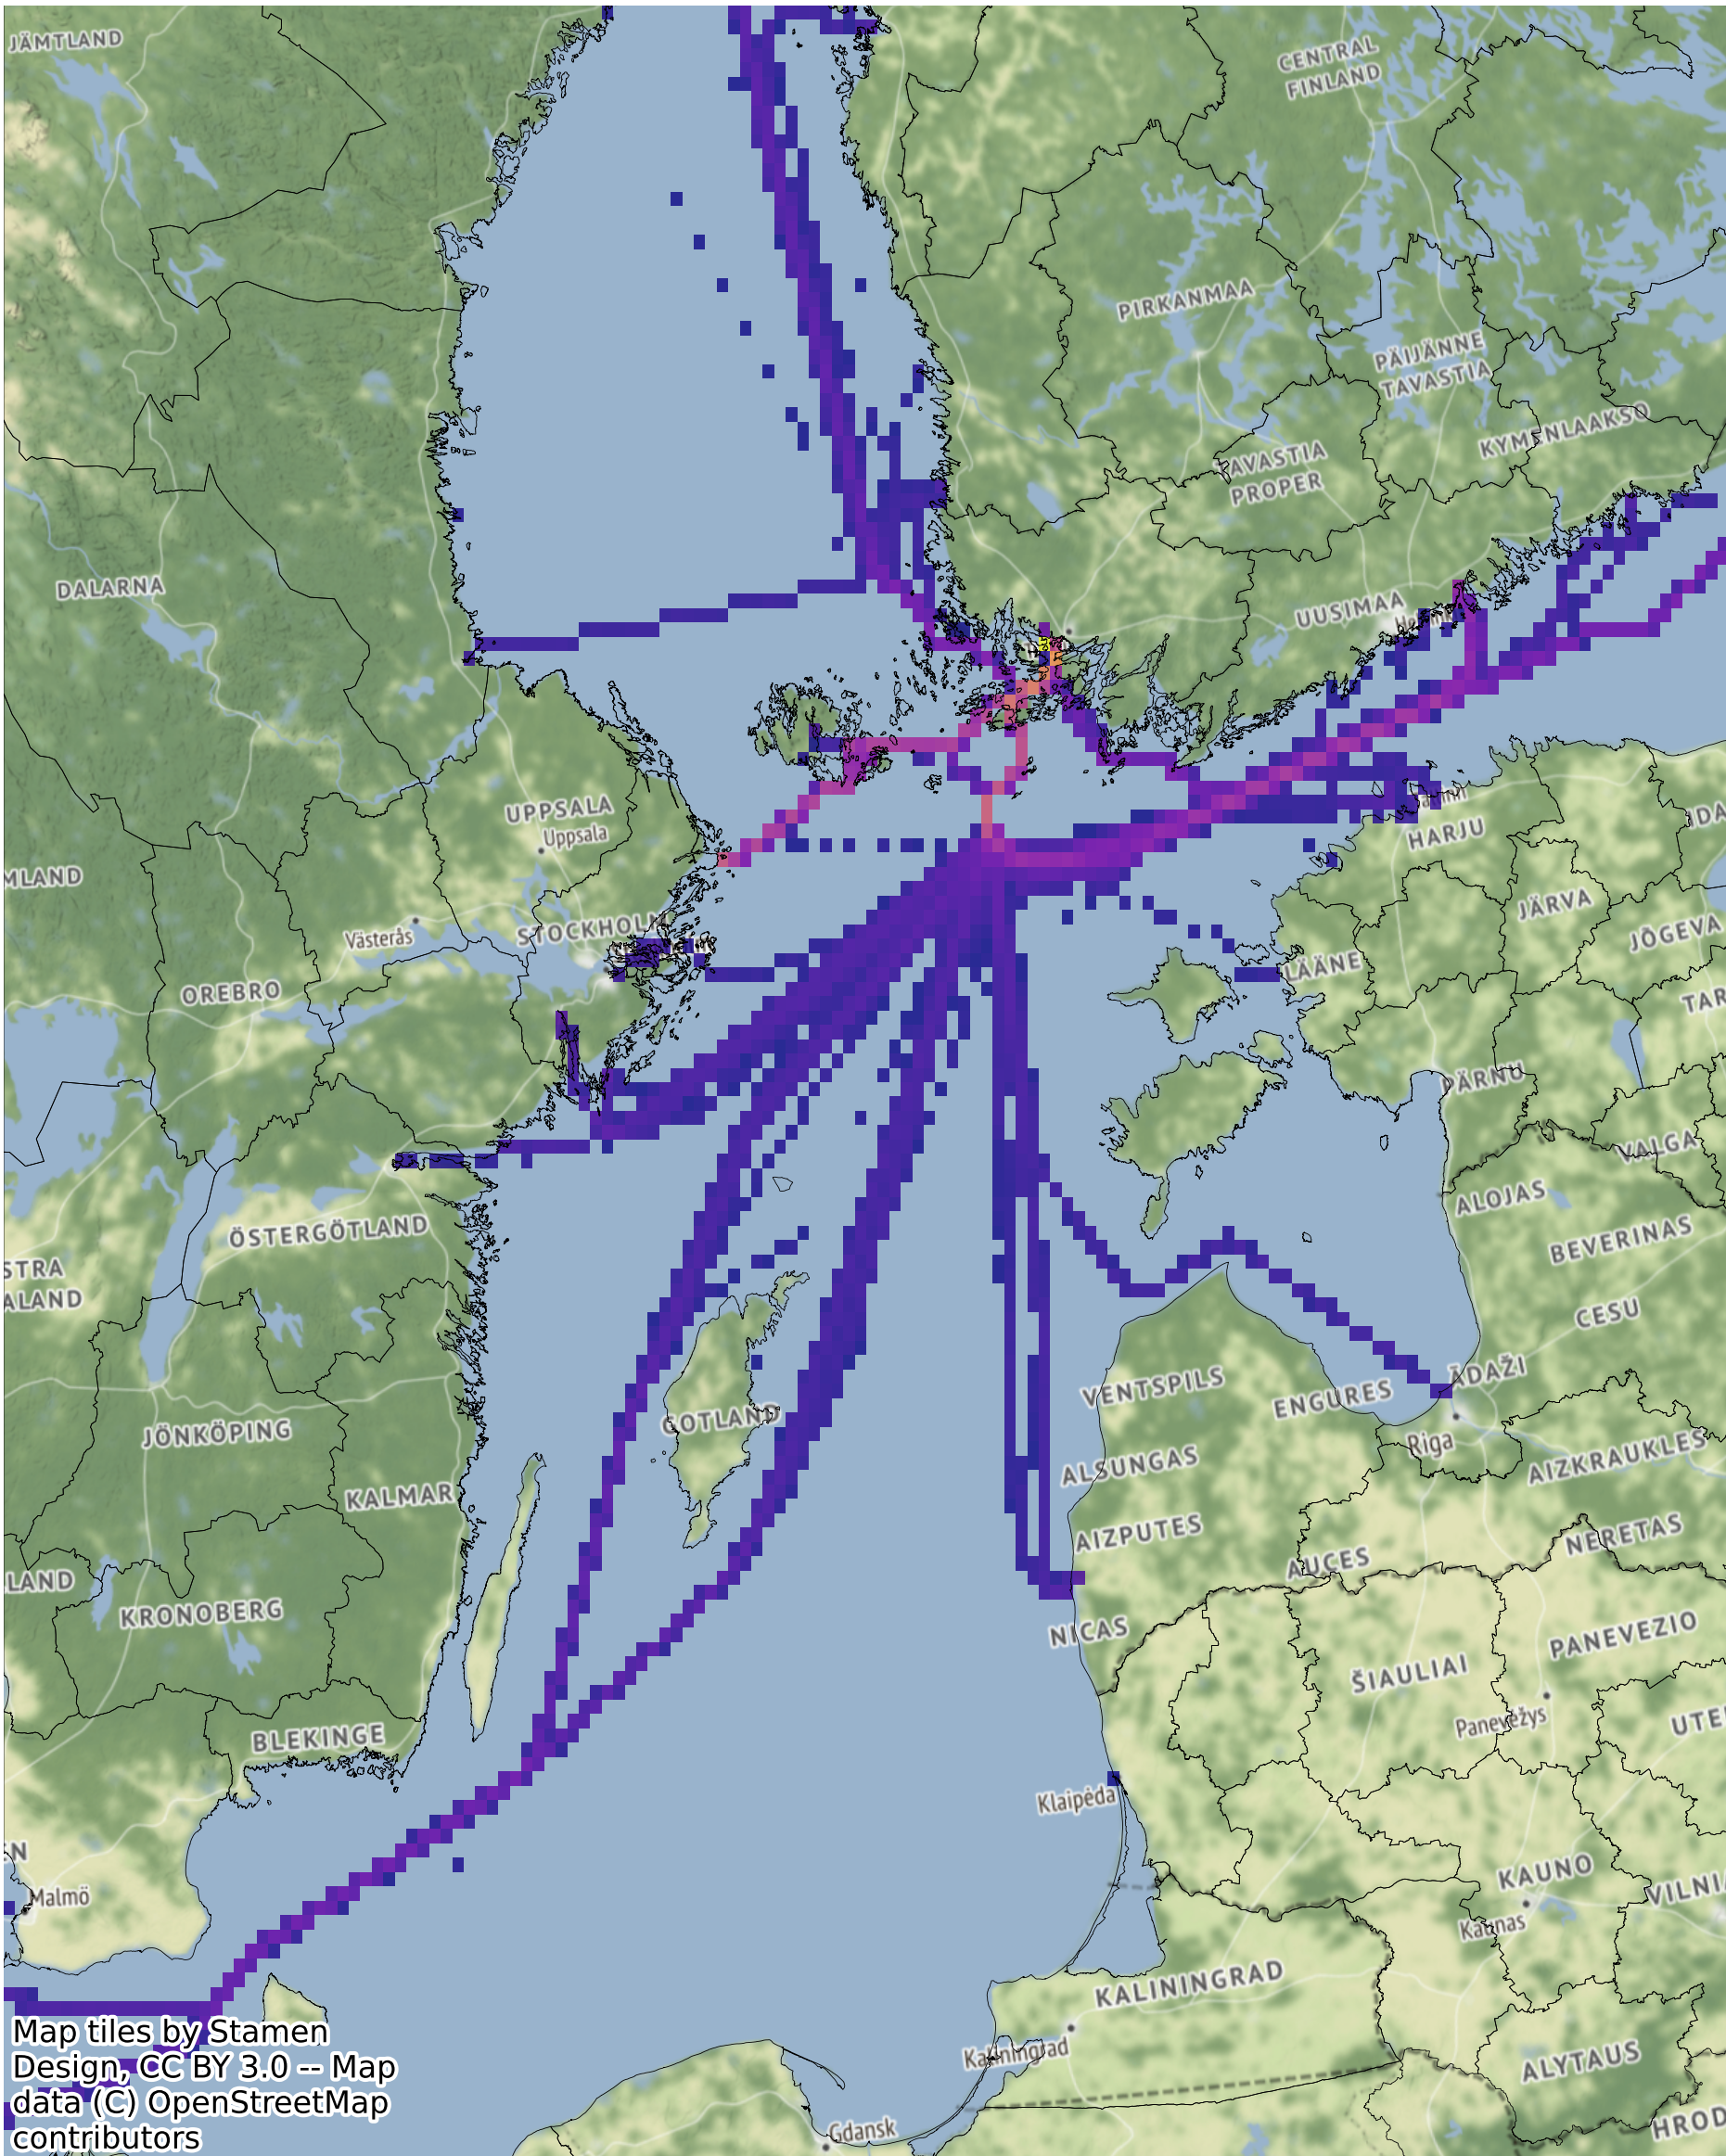
\includegraphics[scale=.3]{heatmap-train-data-13-03.png}
\caption{Heatmap the Baltic Sea with a limit of more than 10 unique messages per grid cell.}
\label{fig:heatmap}
\end{figure}

\subsubsection{Description of HELCOM dataset features}

The HELCOM dataset have twelve unique features for each entry described in Table \ref{tabl:HELCOM-features}. There are bad rows in the dataset, i.e. rows that have a or many bad values.

\begin{table}[H]
\centering
\begin{tabular}{|l|m{7cm}|l|}
\hline
\textbf{Name} & \textbf{Description}                                                  & \textbf{Value}             \\ \hline
timestamp     & Unix epoch time in milliseconds when AIS message was created          & Min 1230768000000          \\ \hline
mmsi          & Maritime Mobile Service Identities, unique for each vessel can change & 9 digits long              \\ \hline
lat           & Latitude position when AIS message was generated                      & Coordinate in WGS 84       \\ \hline
long          & Longitude position when AIS message was generated                     & Coordinate in WGS 84       \\ \hline
sog           & Speed over ground in knots                                            & 0.1 knot resolution        \\ \hline
cog           & Course over ground in degrees relative to true north                  & 0.1 degrees                \\ \hline
draught       & Vertical distance from waterline to the keel                          & 0.1 meters                 \\ \hline
dimBow        & Reference point for position of positioning system on the vessel      & Meters from bow            \\ \hline
dimPort       & Reference point for position of positioning system on the vessel      & Meters from port side      \\ \hline
dimStarboard  & Reference point for position of positioning system on the vessel      & Meters from starboard side \\ \hline
dimStern      & Reference point for position of positioning system on the vessel      & Meters from stern          \\ \hline
imo           & Unique identifier for each vessel, does not change                    & 7 digit identifier         \\ \hline
\end{tabular}
\caption{Variables in HELCOM data set and description.}
\label{tabl:HELCOM-features}
\end{table}

\subsubsection{Statistical information}

Unevenness of the recorded messages (time intervals distribution even) but large gaps in routes. Reasons can be merging of many databases, preprocessing of the data to unify the records. The number of "good" valid routes for training is much lower than the total number of routes. Some of that could be handled by generating routes (data) where there are gaps. In a realistic dataset with AIS data there are going to be faulty data and missing, so HELCOM data is quite accurate to real data without generating missing data.

Vessels physical features and the grouping of different vessels by size.

\subsection{Port of Naantali}

The amount of data collected travelling to FINLI from the HELCOM dataset, rather busy port approx. 2 \% of the total data per month

The projects definition of the port, the bounding box with image.

\end{document}